\section{Introduction}
\label{sec:introduction}

%\begin{figure}
%  \centering
%  \begin{subfigure}[b]{0.25\textwidth}
%    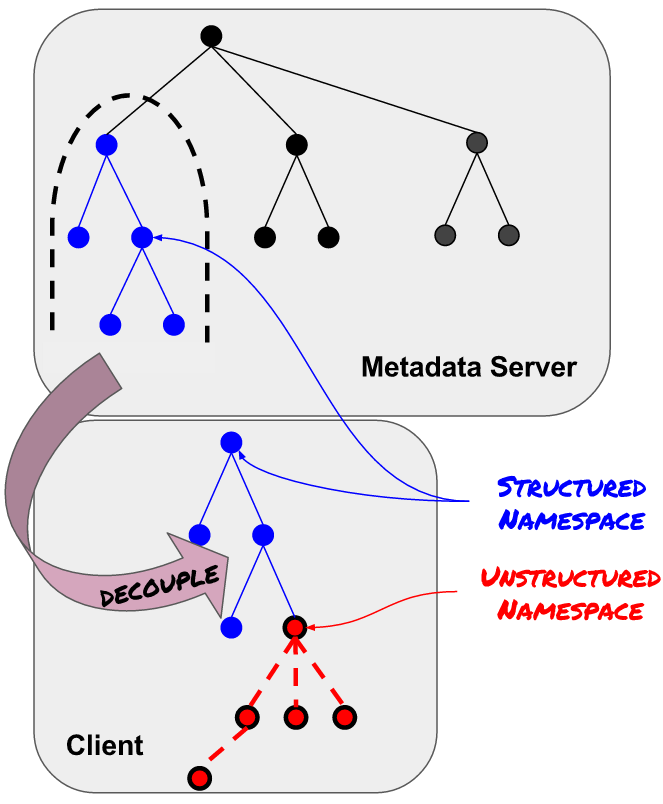
\includegraphics[width=\textwidth]{figures/intro.png}
%   \label{fig:intro}
%  \end{subfigure}
%  ~ 
%  \begin{subfigure}[b]{0.3\textwidth}
%    \begin{tabular}{ r | l }
%      Type         & Overhead       \\\hline\\
%      Structured   & 1 RPC          \\
%      Namespace    & O(1)           \\\\\hdashline\\
%      Unstructured & 1 RPC + Replay \\
%      Namespace    & O(1)           \\\\\hdashline\\
%      Traditional  & \(n\) RPCs     \\
%      Namespace    & O(\(n\))       \\
%    \end{tabular}
%    \\\\\\ % I am a hack
%   \label{table:intro}
%  \end{subfigure}
%  \caption{Clients decouple the file system subtrees and interact with their
%  private copiese locally for high performance. They can specify the structure of
%  the metadata they intend to create (structured namespace) or they can create
%  ad-hoc metadata (unstructured namespace), which is merged later.}
%\end{figure}
%    \caption{Traditional namespaces require at least 1 RPC per metadata
%    operation. Structured namespaces only need the initial RPC so clients/servers
%    understand (and can construct) the namespace.  Unstructured namespaces cannot
%    be parallelized and must replay metadata one by one onto the global namespace}
 
% What is our solution
We propose Tintenfisch, a file system that allows users to succinctly express
the structure and patterns of the metadata they intend to create.  They can
also merge new metadata (that they did not explicitly state up front) into the
global namespace.  Using this semantic knowledge, Tintenfisch can optimize
performance by reducing the number of RPCs needed for (1) metadata writes
because clients/servers can create metadata independently and (2) metadata
reads because clients can construct metadata and pull data directly from the
object store. Figure~\ref{fig:intro} provides an architectural overview;
clients first decouple the file system subtree they want to operate
on\footnote{This is not a contribution as it was presented
in~\cite{sevilla:ipdps18-cudele}.} then clients and metadata servers lazily
generate subtrees as needed using a namespace schema (described
in~\S\ref{sec:namespace-schemas}). The namespace schema is stored in the root
inode of the decoupled subtree.

\begin{figure}[t]
  \centering
  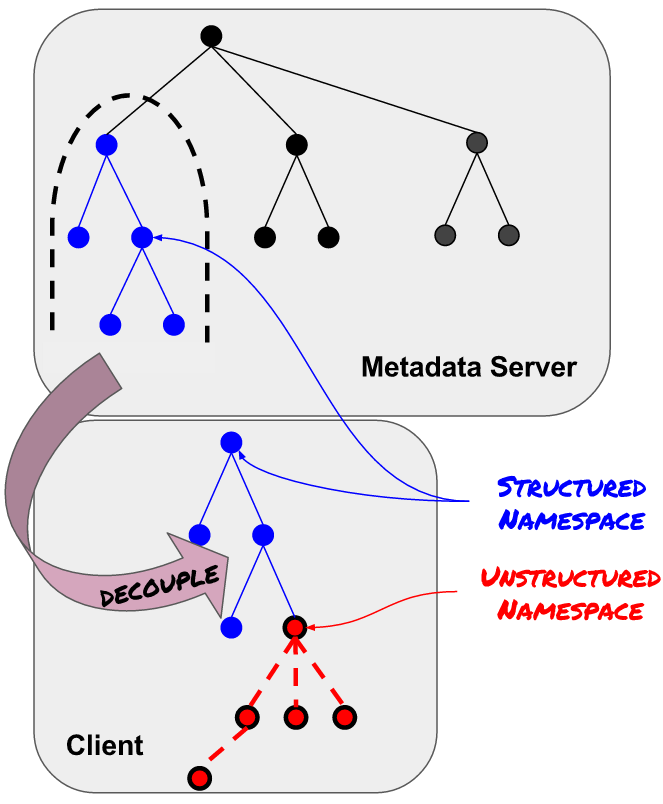
\includegraphics[width=0.9\linewidth]{figures/intro.png}
  \caption{In (1), clients decouple file system subtrees and interact
with their copies locally for high performance. In (2), clients and
metadata servers generate subtrees using ``namespace schemas", thus reducing
RPC load.  \label{fig:intro}}
\end{figure}

The fundamental insight is that the client and server both understand the final
structure of the file system metadata so there is no need to communicate.  The
idea uses concepts from decoupled namespaces~\cite{zheng:pdsw2014-batchfs,
zheng:pdsw2015-deltafs} and patterned IO~\cite{he:hpdc13-plfs-patterns} to
build a scalable global namespace. Less work is done on the metadata servers
and clients pick up some of the metadata load.  This approach is similar to
predicate push downs in databases, where structure is described to lower
storage layers using XML or JSON~\cite{shel:pc17-pushdown}. It is our hope that
Tintenfisch will also be able to change the representation or structure of the
file system metadata according to the file type or workload.  We have the
following contributions:

\begin{itemize}
  \setlength\itemsep{-0.5em}

  \item namespace descriptions and overheads for examples from different
domains (high performance computing, high energy physics, and large scale
simulations)

  \item namespace schemas: a technique to compact metadata, thus reducing RPC
amplification and facilitating lazy metadata generation when needed

  \item a programmable storage approach that pushes user-defined functionality
into the storage system, facilitating application-specific storage stacks using
a `dirty-slate' approach

\end{itemize}
